% Digital Logic Report Template
% Created: 2020-01-10, John Miller

%==========================================================
%=========== Document Setup  ==============================

% Formatting defined by class file
\documentclass[11pt]{article}

% ---- Document formatting ----
\usepackage[margin=1in]{geometry}	% Narrower margins
\usepackage{booktabs}				% Nice formatting of tables
\usepackage{graphicx}				% Ability to include graphics

%\setlength\parindent{0pt}	% Do not indent first line of paragraphs 
\usepackage[parfill]{parskip}		% Line space b/w paragraphs
%	parfill option prevents last line of pgrph from being fully justified

% Parskip package adds too much space around titles, fix with this
\RequirePackage{titlesec}
\titlespacing\section{0pt}{8pt plus 4pt minus 2pt}{3pt plus 2pt minus 2pt}
\titlespacing\subsection{0pt}{4pt plus 4pt minus 2pt}{-2pt plus 2pt minus 2pt}
\titlespacing\subsubsection{0pt}{2pt plus 4pt minus 2pt}{-6pt plus 2pt minus 2pt}

% ---- Hyperlinks ----
\usepackage[colorlinks=true,urlcolor=blue]{hyperref}	% For URL's. Automatically links internal references.

% ---- Code listings ----
\usepackage{listings} 					% Nice code layout and inclusion
\usepackage[usenames,dvipsnames]{xcolor}	% Colors (needs to be defined before using colors)

% Define custom colors for listings
\definecolor{listinggray}{gray}{0.98}		% Listings background color
\definecolor{rulegray}{gray}{0.7}			% Listings rule/frame color

% Style for Verilog
\lstdefinestyle{Verilog}{
	language=Verilog,					% Verilog
	backgroundcolor=\color{listinggray},	% light gray background
	rulecolor=\color{blue}, 			% blue frame lines
	frame=tb,							% lines above & below
	linewidth=\columnwidth, 			% set line width
	basicstyle=\small\ttfamily,	% basic font style that is used for the code	
	breaklines=true, 					% allow breaking across columns/pages
	tabsize=3,							% set tab size
	commentstyle=\color{gray},	% comments in italic 
	stringstyle=\upshape,				% strings are printed in normal font
	showspaces=false,					% don't underscore spaces
}

% How to use: \Verilog[listing_options]{file}
\newcommand{\Verilog}[2][]{%
	\lstinputlisting[style=Verilog,#1]{#2}
}




%======================================================
%=========== Body  ====================================
\begin{document}

\title{ELC 2137 Lab 11: Lab 11 FSM: Guessing Game}
\author{Makenna Meyers}

\maketitle


\section*{Summary}
 This lab uses a Finite State Machine (FSM) to develop a game in which irregular, non-repeating conditions are used. The code used can be found in Listings \ref{code:gfsm}, \ref{code:gfsm_test}, \ref{code:guessing_game}. 
 
 \section*{Q/A}
 \begin{enumerate}
 	
 	\item At what time in the simulation did the debounce circuit reach each of the four states (zero, wait1, one, wait0)?
 	
 	Zero was reached at 0 ns and 645 ns, wait 1 was reached at 200 ns, one was reached at 245 ns, and wait 0 was reached at 600 ns.
 	
 	\item Why can this game not be implemented with regular sequential logic?
 	
 	This design involves irregular, non-repeating conditions that cannot be described with regular sequential logic.
 	
 	\item What type of outputs did you use for your design? Mealy or Moore? Explain.
 	
 	Mealy outputs were used because the output depends on both the present state and the present input. Moore outputs rely only on the present state.
 	
 \end{enumerate}


\section*{Results}

\begin{figure}[ht]\centering
	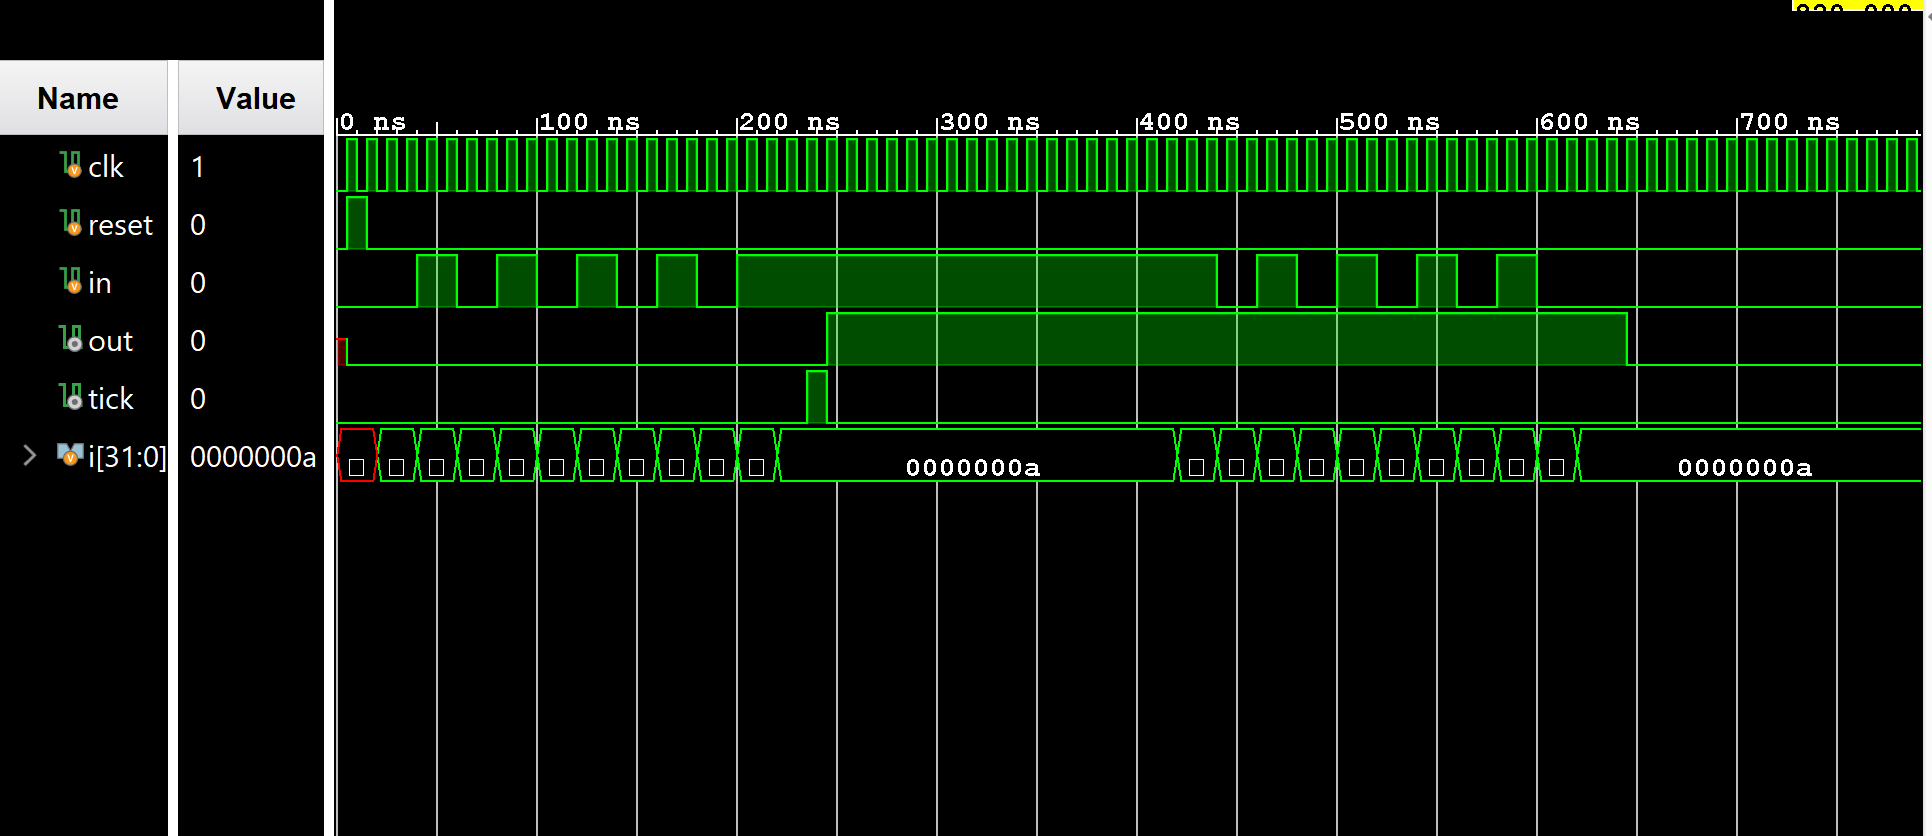
\includegraphics[width=0.8\textwidth,trim=0cm 0cm 0cm 0cm,clip]{debounce_simwave}
	\caption{Debounce Simulation Waveform}
	\label{fig:debounce_simwave}			
\end{figure}
\clearpage

	
\section*{Code}

\Verilog[caption=Guess FSM Module,label=code:gfsm]{guess_FSM.sv}

\Verilog[caption=Guess FSM Test Bench,label=code:gfsm_test]{guess_FSM_test.sv}

\Verilog[caption=Guessing Game Module,label=code:guessing_game]{guessing_game.sv}


\end{document}